% Options for packages loaded elsewhere
\PassOptionsToPackage{unicode}{hyperref}
\PassOptionsToPackage{hyphens}{url}
%
\documentclass[
]{article}
\usepackage{amsmath,amssymb}
\usepackage{iftex}
\ifPDFTeX
  \usepackage[T1]{fontenc}
  \usepackage[utf8]{inputenc}
  \usepackage{textcomp} % provide euro and other symbols
\else % if luatex or xetex
  \usepackage{unicode-math} % this also loads fontspec
  \defaultfontfeatures{Scale=MatchLowercase}
  \defaultfontfeatures[\rmfamily]{Ligatures=TeX,Scale=1}
\fi
\usepackage{lmodern}
\ifPDFTeX\else
  % xetex/luatex font selection
\fi
% Use upquote if available, for straight quotes in verbatim environments
\IfFileExists{upquote.sty}{\usepackage{upquote}}{}
\IfFileExists{microtype.sty}{% use microtype if available
  \usepackage[]{microtype}
  \UseMicrotypeSet[protrusion]{basicmath} % disable protrusion for tt fonts
}{}
\makeatletter
\@ifundefined{KOMAClassName}{% if non-KOMA class
  \IfFileExists{parskip.sty}{%
    \usepackage{parskip}
  }{% else
    \setlength{\parindent}{0pt}
    \setlength{\parskip}{6pt plus 2pt minus 1pt}}
}{% if KOMA class
  \KOMAoptions{parskip=half}}
\makeatother
\usepackage{xcolor}
\usepackage[margin=1in]{geometry}
\usepackage{graphicx}
\makeatletter
\def\maxwidth{\ifdim\Gin@nat@width>\linewidth\linewidth\else\Gin@nat@width\fi}
\def\maxheight{\ifdim\Gin@nat@height>\textheight\textheight\else\Gin@nat@height\fi}
\makeatother
% Scale images if necessary, so that they will not overflow the page
% margins by default, and it is still possible to overwrite the defaults
% using explicit options in \includegraphics[width, height, ...]{}
\setkeys{Gin}{width=\maxwidth,height=\maxheight,keepaspectratio}
% Set default figure placement to htbp
\makeatletter
\def\fps@figure{htbp}
\makeatother
\setlength{\emergencystretch}{3em} % prevent overfull lines
\providecommand{\tightlist}{%
  \setlength{\itemsep}{0pt}\setlength{\parskip}{0pt}}
\setcounter{secnumdepth}{-\maxdimen} % remove section numbering
\ifLuaTeX
  \usepackage{selnolig}  % disable illegal ligatures
\fi
\IfFileExists{bookmark.sty}{\usepackage{bookmark}}{\usepackage{hyperref}}
\IfFileExists{xurl.sty}{\usepackage{xurl}}{} % add URL line breaks if available
\urlstyle{same}
\hypersetup{
  pdftitle={Análisis de la dinámica empresarial en Ecuador.},
  pdfauthor={Geovanna Gonzalez},
  hidelinks,
  pdfcreator={LaTeX via pandoc}}

\title{Análisis de la dinámica empresarial en Ecuador.}
\author{Geovanna Gonzalez}
\date{2023-09-11}

\begin{document}
\maketitle

\hypertarget{resumen-ejecutivo.}{%
\subsection{\texorpdfstring{\textbf{Resumen
ejecutivo.}}{Resumen ejecutivo.}}\label{resumen-ejecutivo.}}

El Directorio de Compañías de la Superintendencia de Compañías, Valores
y Seguros (SCVS) del Ecuador es una base de datos fundamental y pública
que contiene información sobre las empresas y organizaciones registradas
en Ecuador. La Superintendencia de Compañías es una entidad encargada de
regular y supervisar la actividad empresarial, y su directorio es una
fuente invaluable de datos para el sector empresarial, el gobierno y
otros interesados.

A lo largo de décadas, Ecuador ha experimentado un notable cambio en la
dirección de compañías. Desde 1.968, se ha observado un crecimiento
constante en la creación de nuevas empresas, alcanzando un punto
culminante en 2022 con la incorporación de 19.514 compañías. Esto
resalta un ferviente espíritu emprendedor en el país.

Un dato significativo es la distribución temporal de esta actividad.
Marzo emergió como el mes estrella para la creación de empresas en los
años 2022 y 2023, sugiriendo patrones estacionales o factores
desencadenantes específicos en esos momentos.

En el contexto provincial, Guayas lidera en promedio la creación de
empresas, con un promedio de 7.724 compañías registradas, seguido de
cerca por Pichincha, con 6.020. Esta diferencia en la actividad
empresarial entre las provincias es notable y podría estar relacionada
con factores geográficos, económicos y demográficos.

Un enfoque adicional revela las actividades comerciales predominantes en
estas provincias. Guayas se destaca en el comercio al por mayor y al por
menor, así como en la reparación de vehículos automotores y
motocicletas. Pichincha, por otro lado, muestra una fuerte presencia en
el comercio y reparación de vehículos. Estos datos ofrecen una visión
más detallada de las áreas económicas en las que cada provincia se
destaca, lo que puede ser esencial para la toma de decisiones
empresariales y políticas económicas.

\hypertarget{desarrollo}{%
\subsection{\texorpdfstring{\textbf{Desarrollo}}{Desarrollo}}\label{desarrollo}}

El presente informe analiza la situación actual y las tendencias en la
creación y distribución de empresas en Ecuador,así también, busca
comprender mejor la actividad económica y empresarial en el país
mediante consultas y análisis específicos en la base de datos de la
Superintendencia de Compañías del Ecuador.

Las empresas activas son aquellas que está operando y funcionando en la
actualidad. Es decir, es una entidad comercial que está en
funcionamiento y que realiza actividades económicas regulares, como la
producción, la prestación de servicios o la venta de productos, etc.

A continuación se presenta un gráfico que ilustra el total de empresas
activas en diferentes periodos, antes y luego de la pandemia.

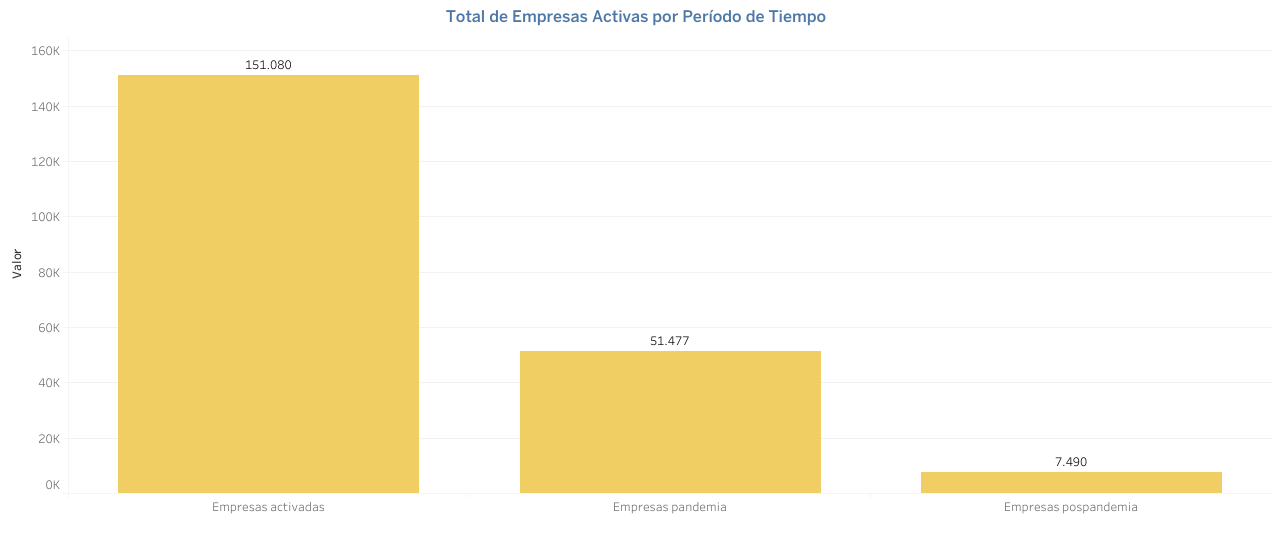
\includegraphics{imagenes/Hoja 2 (1).png}

El gráfico 1 presenta la dinámica de creación de empresas en el tiempo.
Durante la pandemia, pese que varias compañias cerraron, otras iniciaron
su vida comercial, se observa que 51.477 empresas emergieron en la
crisis sanitaria, lo que refleja una respuesta empresarial a las
circunstancias cambiantes. Sin embargo, tras la pandemia, se registra
una marcada disminución, de 7.490 empresas, lo que podría estar
relacionado con factores económicos y de mercado. Esta representación
visual destaca la volatilidad en la actividad empresarial y cómo los
eventos globales pueden tener un impacto en la formación y el cierre de
empresas en un corto período de tiempo.

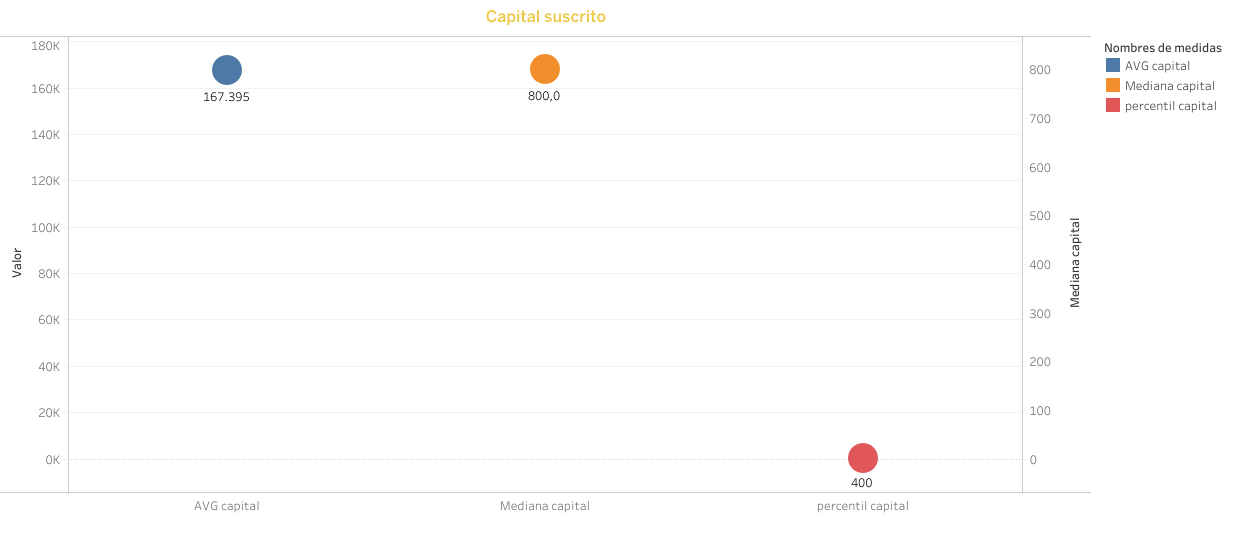
\includegraphics{imagenes/Hoja 3.png}

En el gráfico indica el promedio del capital suscrito que es de 167.395.
Esto significa que, en promedio, las empresas en el conjunto de datos
tienen un capital suscrito de alrededor de 167.395 unidades monetarias.
El promedio se calcula sumando todos los valores de capital suscrito y
dividiéndolos por el número de empresas.La mediana del capital suscrito
es de 800. La mediana es el valor que se encuentra justo en el medio de
todos los valores cuando están ordenados de menor a mayor. En este caso,
el valor de 800 es el punto medio, lo que sugiere que aproximadamente la
mitad de las empresas tienen un capital suscrito por debajo de 800 y la
otra mitad por encima de 800. El valor obtenido, que es 400, indica que
el 20\% de las empresas en el conjunto de datos tienen un capital
suscrito igual o inferior a 400 unidades monetarias. Esto proporciona
información sobre la distribución de los valores en el conjunto de datos
y destaca que un segmento significativo de las empresas tiene un capital
suscrito relativamente bajo.

La CIIU ``Clasificación Industrial Internacional Uniforme'' se compone
de una serie de códigos y categorías numéricas que representan
diferentes tipos de actividades económicas, como la agricultura, la
manufactura, los servicios, la construcción, entre otros. Estos códigos
se organizan jerárquicamente en varios niveles, lo que permite una
clasificación detallada de las actividades económicas a nivel global.

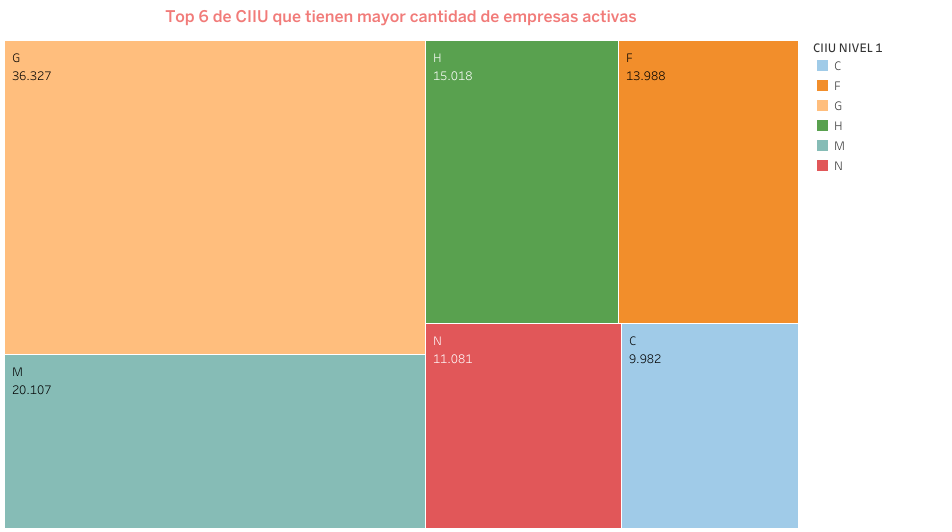
\includegraphics{imagenes/Hoja 4.png}

La gráfica 3 muestra las 6 actividades económicas con mayor empresas
activas. En primer lugar, ``Comercio al por Mayor y al por Menor;
Reparación de Vehículos de Automotores y Motocicletas'' (Código G)
lidera con 36,327 compañías, lo que subraya la importancia del comercio
en el país. En segundo lugar, ``Actividades Profesionales, Científicas y
Técnicas'' (Código M) cuenta con 20,107 empresas activas, indicando una
presencia significativa de servicios profesionales y técnicos. El sector
de ``Transporte y Almacenamiento'' (Código H) ocupa el tercer lugar con
15,018 empresas activas, mientras que ``Construcción'' (Código F) se
ubica en el cuarto lugar con 13,988 compañías, destacando la robustez de
la industria de la construcción. ``Actividades de Servicios
Administrativos y de Apoyo'' (Código N) se encuentra en el quinto lugar,
con 11,081 empresas activas, y ``Industrias Manufactureras'' (Código C)
completa la lista en el sexto lugar, con 9,982 empresas activas. Esta
diversidad en las actividades económicas resalta la vitalidad y el
potencial de la economía ecuatoriana, brindando oportunidades en varios
sectores para el crecimiento empresarial y la inversión. Este análisis
muestra una diversidad de actividades económicas activas en Ecuador, con
un fuerte énfasis en el comercio, los servicios profesionales, el
transporte, la construcción y las industrias manufactureras. Estos
sectores desempeñan un papel importante en la economía del país y
ofrecen oportunidades para el crecimiento empresarial y la inversión.

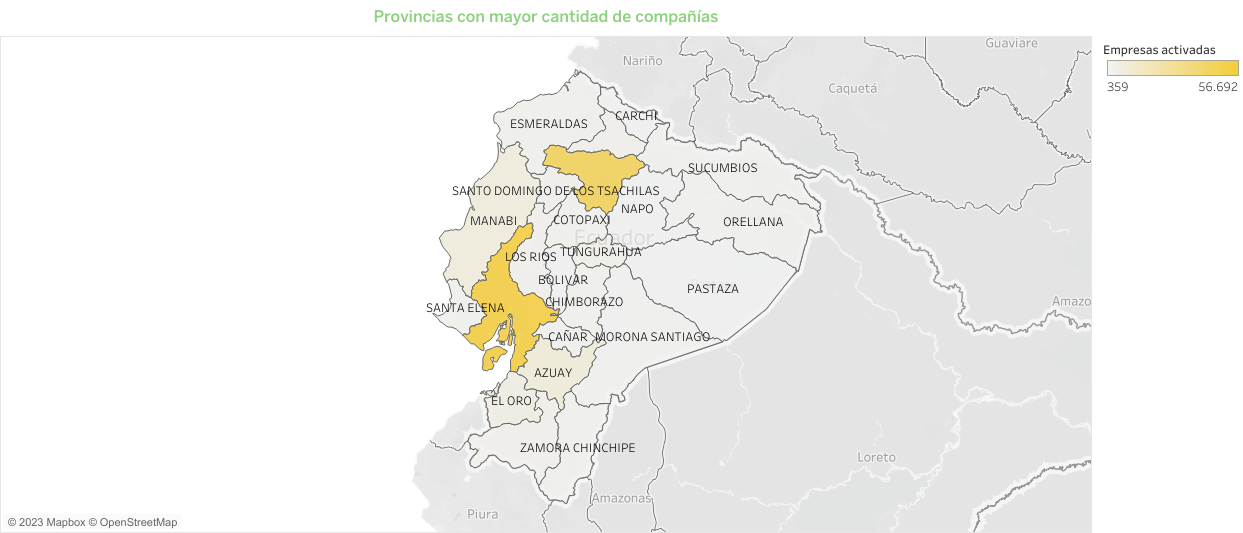
\includegraphics{imagenes/Hoja 5.png}

La gráfica destaca las provincias de Pichincha y Guayas como líderes en
la cantidad de compañías registradas en Ecuador, con 49,000 y 56,692
empresas respectivamente. Pichincha, que incluye la capital Quito, se
destaca como un importante centro económico y empresarial, mientras que
Guayas, que alberga la ciudad portuaria de Guayaquil, muestra una
impresionante concentración de empresas en la región costera del país.
Esta ilustración resalta la relevancia económica y comercial de estas
dos provincias en la estructura empresarial de Ecuador.

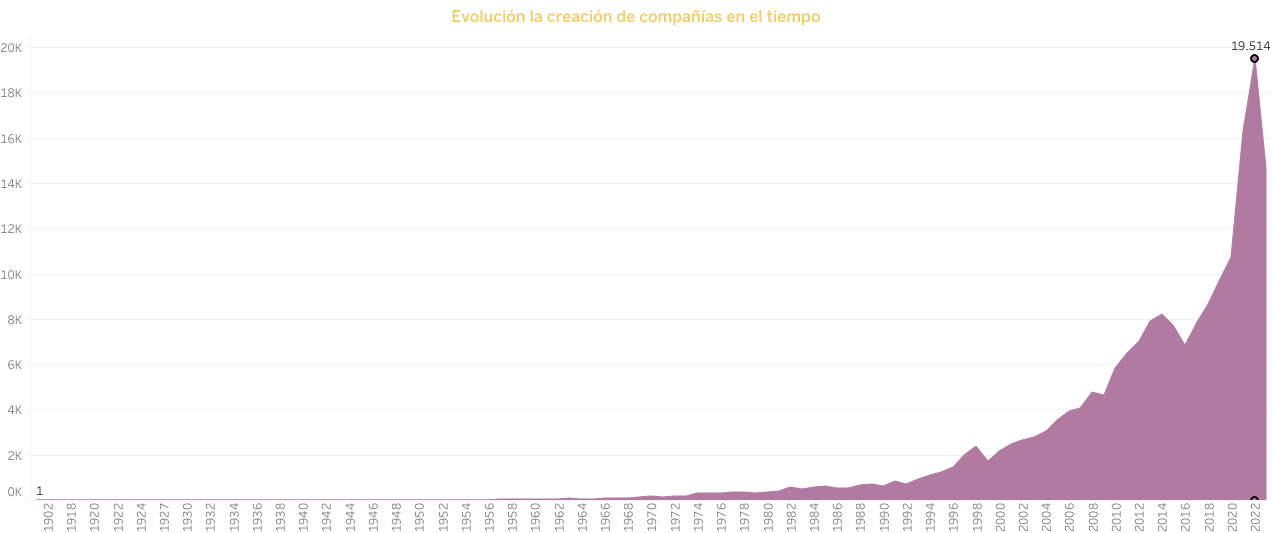
\includegraphics{imagenes/Hoja 11.png}

La evolución de la creación de compañías a lo largo del tiempo revela un
patrón interesante en el que, en 1902, solo se registró una empresa,
marcando un comienzo modesto. Durante las décadas siguientes, la
cantidad de empresas aumentó gradualmente pero se mantuvo en niveles
bajos, hasta que en 1968 se produjo un punto de inflexión con un total
de 110 empresas registradas, indicando un crecimiento significativo en
la actividad empresarial. A partir de ese año, la tendencia fue al alza,
sugiriendo posibles cambios económicos, regulatorios o de espíritu
empresarial. El año 2022 se destacó con un récord de 19.514 empresas
registradas, posiblemente debido a factores como oportunidades de
mercado, inversiones y políticas gubernamentales que influyeron en la
creación de empresas en la región.

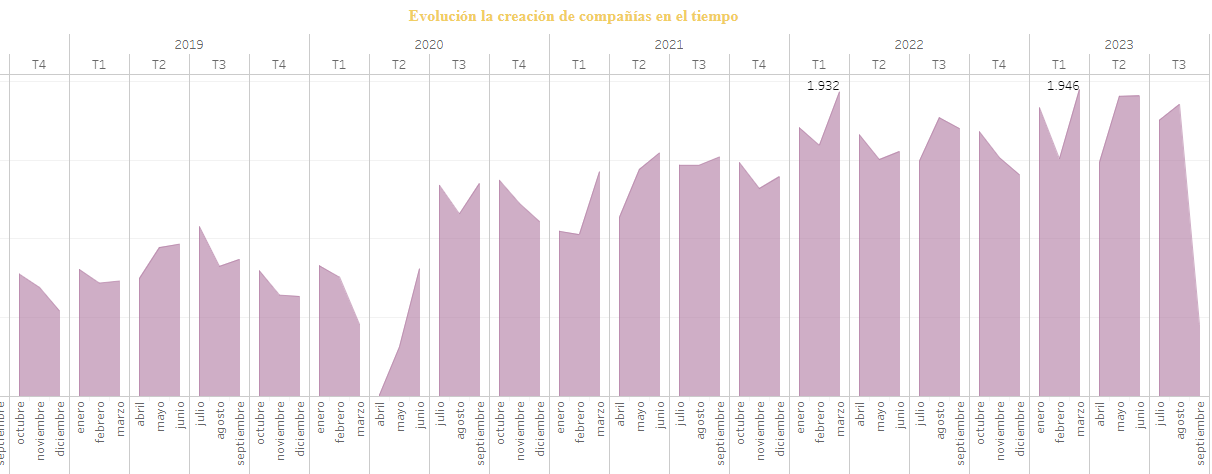
\includegraphics{imagenes/GGBB.png}

En el análisis mensual de la creación de compañías, se observa que los
meses de marzo tanto en 2022 como en 2023 destacan como los períodos en
los que se crean la mayor cantidad de empresas, con 1.932 y 1.946
empresas registradas, respectivamente. Estos dos puntos altos en marzo
sugieren un patrón de actividad empresarial estacional con un fuerte
impulso en la creación de empresas durante ese mes en los años
mencionados.

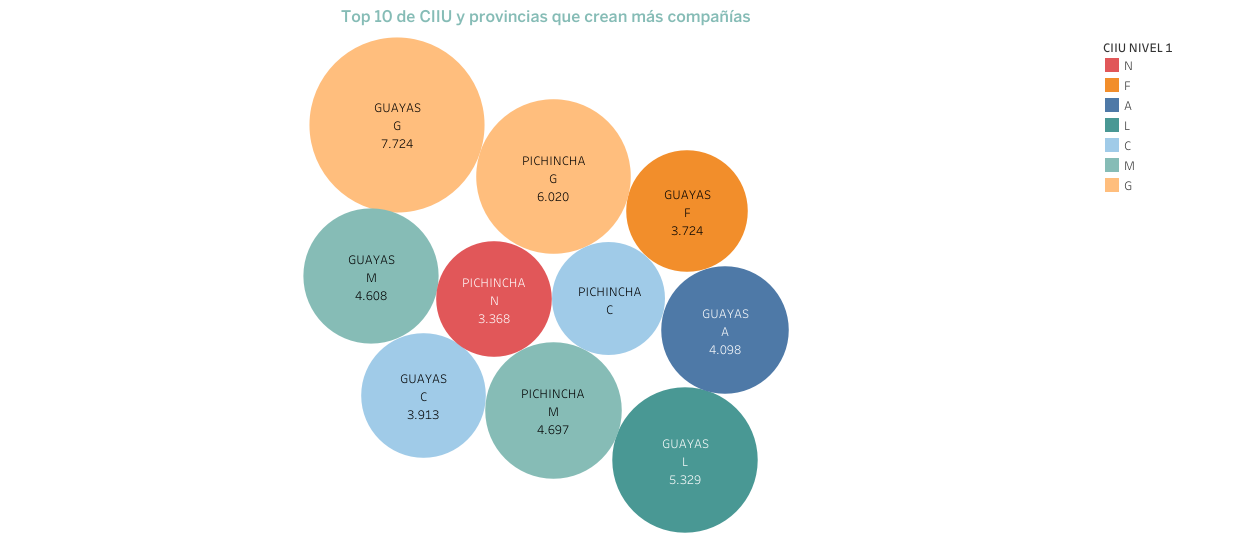
\includegraphics{imagenes/Hoja 7.png}

En promedio, las actividades comerciales (CIIU) que generan más
compañías en Ecuador son aquellas asociadas al sector G, que incluye el
comercio al por mayor y al por menor, junto con la reparación de
vehículos automotores y motocicletas, con valores notables en Guayas
(7.724 empresas) y Pichincha (6.020 empresas). Por otro lado, las
actividades relacionadas con la construcción (F) muestran un promedio
más bajo en ambas provincias, con 3.724 empresas en Guayas y 3.216 en
Pichincha. Estos datos resaltan la importancia de estos sectores en la
creación de empresas y ofrecen una visión de las dinámicas empresariales
en el país.

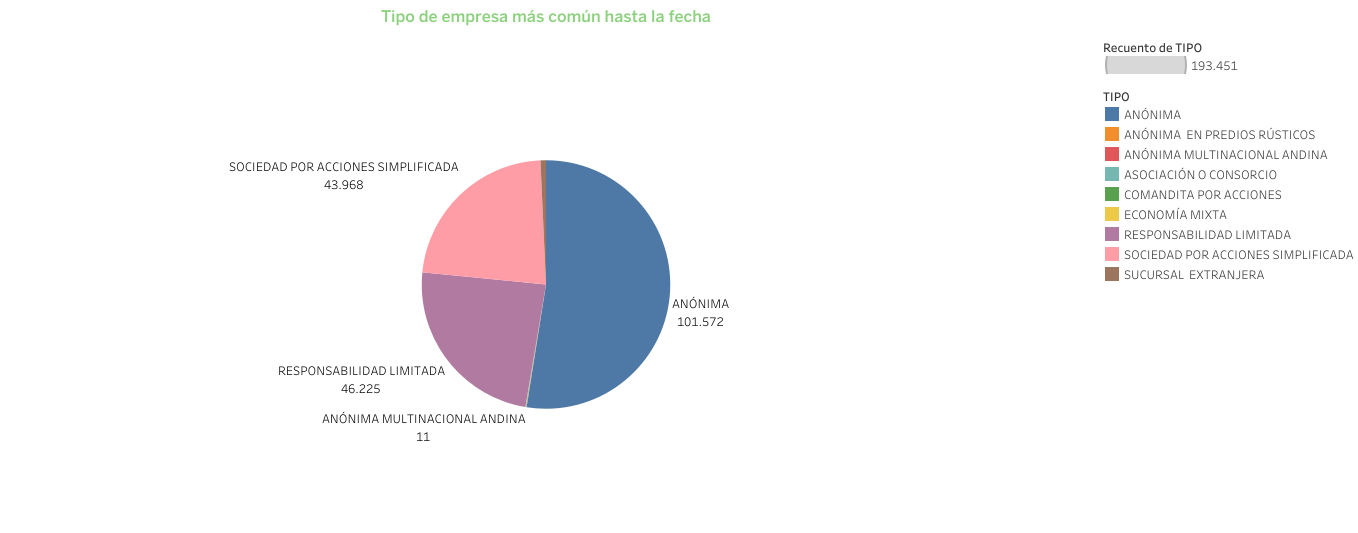
\includegraphics{imagenes/Hoja 8.png}

En Ecuador las sociedades anónimas son el tipo de empresa más común
hasta la fecha, con un total de 101.572 registros, seguidas por las
sociedades de responsabilidad limitada, que cuentan con 46.225
registros. Las Sociedades por Acciones Simplificadas (SAS) son menos
comunes en comparación con las otras dos categorías, con un total de
43.968 registros. Por último, las sociedades anónimas multinacionales
andinas son la categoría menos común, con solo 11 registros. Estos
números sugieren que las empresas de estructura anónima y de
responsabilidad limitada son las opciones más preferidas en Ecuador,
mientras que las SAS y las multinacionales andinas tienen una presencia
más limitada en el mercado empresarial del país.

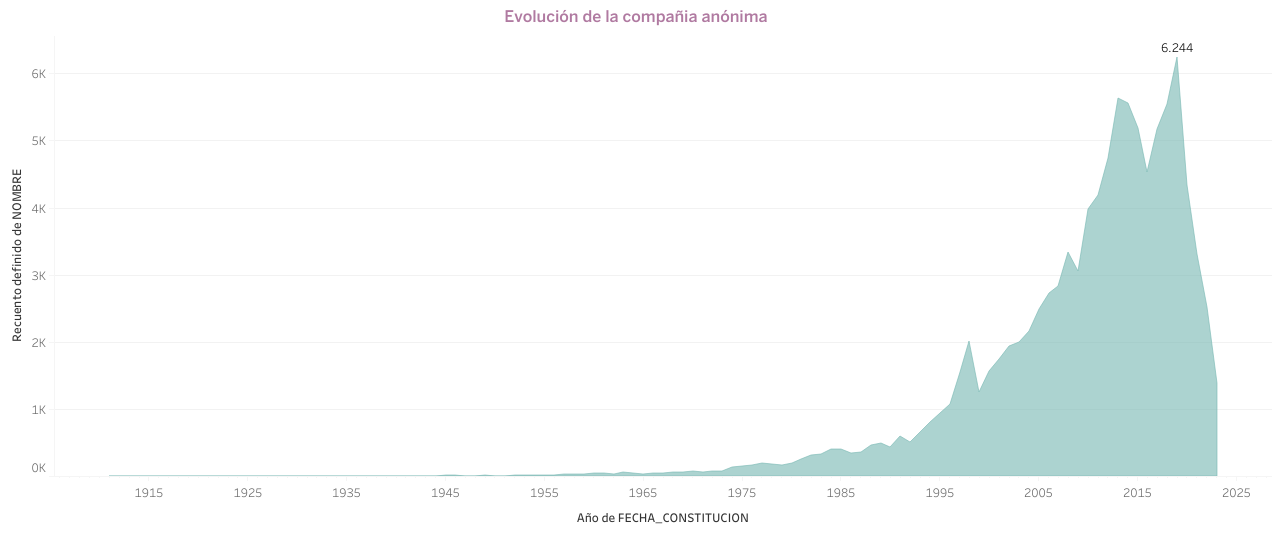
\includegraphics{imagenes/Hoja 9.png}

La evolución del tipo de empresa más común en Ecuador, muestran un
patrón interesante. A lo largo de los años, se observa un aumento
constante en el número de sociedades anónimas registradas. En 1974,
estas empresas superaron las 100, marcando el comienzo de un crecimiento
progresivo. Aunque hay algunas disminuciones en el número de empresas en
años posteriores, no son tan frecuentes ni significativas. Sin embargo,
en 2019, se alcanzó el pico más alto con 6.244 sociedades anónimas
registradas. Luego, en 2023, se observa una disminución pronunciada a
1.385, lo que podría indicar factores económicos, legales o de mercado
que influyeron en esta reducción significativa. En general, la tendencia
a largo plazo muestra un aumento en la popularidad de las sociedades
anónimas en Ecuador, pero con fluctuaciones notables en años más
recientes.

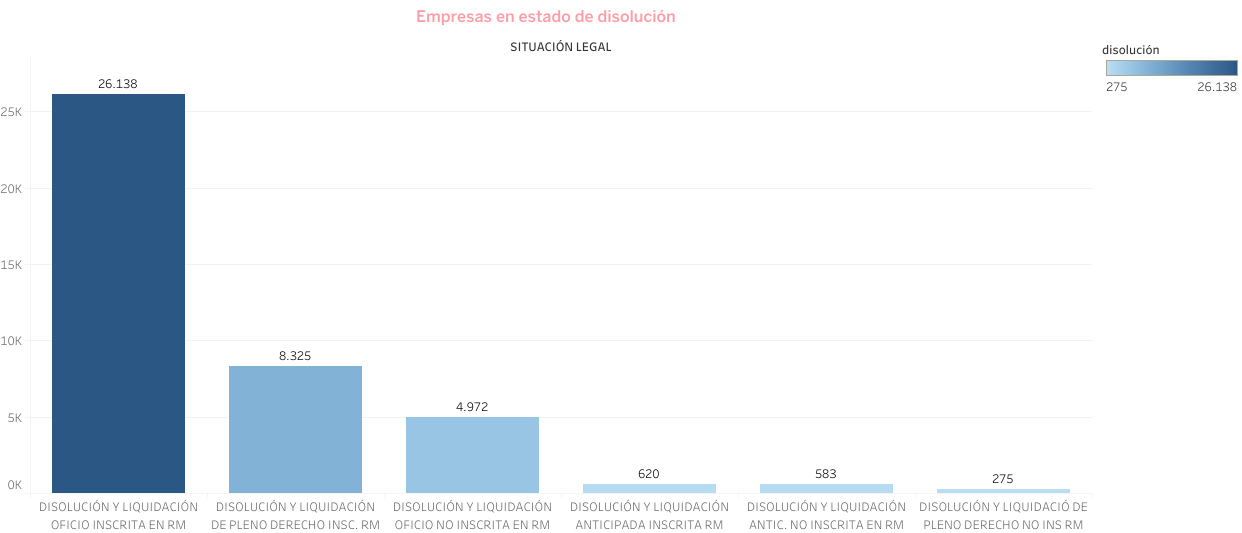
\includegraphics{imagenes/Hoja 10.png}

En la gráfica observado un total de 40.913 empresas en proceso de
disolución en este momento. Estas se dividen en varias categorías, con
la mayoría (26.138) en el estado de ``disolución y liquidación oficio
inscrita en RM'', seguidas por ``disolución y liquidación de pleno
derecho insc. Rm'' con 8.325, ``disolución y liquidación anticipada
inscrita RM'' con 620, ``disolución y liquidación oficio no inscrita en
RM'' con 4.972, ``disolución y liquidación de pleno derecho no ins RM''
con 275 y ``disolución y liquidación antic. No inscrita en RM'' con 583.
Estos datos reflejan una variedad de situaciones en las que las empresas
están en proceso de disolución en diferentes estados y condiciones
legales.

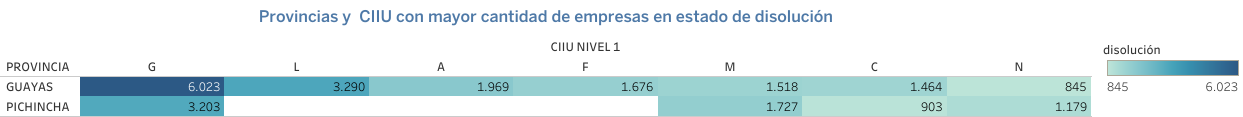
\includegraphics{imagenes/Hoja 10 (2).png}

Como se analizó anteriormente tanto las provincias de Guayas y Pichincha
son aquellas con mayor número de compañias creadas pero tambien destacan
como las regiones con la mayor cantidad de empresas en estado de
disolución en Ecuador. En Guayas, las actividades comerciales
relacionadas con el sector G, que abarca el comercio al por mayor y al
por menor, junto con la reparación de vehículos automotores y
motocicletas, registran 6.023 empresas en estado de disolución, mientras
que en Pichincha, el sector G también lidera con 3.203 empresas en la
misma condición. Además, en Guayas, las actividades relacionadas con la
agricultura (A) y la construcción (F) presentan 1.969 y 1.676 empresas
en estado de disolución, respectivamente, mientras que en Pichincha, las
actividades profesionales, científicas y técnicas (M) y el comercio al
por mayor y al por menor (C) tienen 1.727 y 903 empresas en esta
situación. Esto ofrece una visión importante de las áreas donde las
empresas enfrentan mayores dificultades y resaltan la necesidad de
comprender las causas detrás de la disolución empresarial en estos
sectores.

Finalamente, este análisis integral de las tendencias en la dirección de
compañías en Ecuador destaca el continuo crecimiento de la actividad
empresarial en el país, con algunos puntos culminantes en años
recientes. Además, muestra la variabilidad regional en la creación de
empresas y las actividades comerciales predominantes en cada provincia,
lo que brinda información valiosa para comprender mejor la dinámica
empresarial en Ecuador y orientar futuras estrategias económicas y
empresariales.

\end{document}
